\documentclass[11pt,a4paper,twocolumn]{article}
\usepackage{fancyhdr}
\usepackage[scaled]{helvet} 
\usepackage{amsmath}
\usepackage{cite}
\usepackage{graphicx}
\usepackage{fancybox}
\usepackage{color}
\usepackage[format=hang]{caption}
\usepackage{wrapfig}
\usepackage{tabularx}
\usepackage{framed}
\usepackage{fancyhdr}
\usepackage[parfill]{parskip}
\usepackage{pdflscape}
\usepackage{url}
\usepackage{multirow}
\usepackage{multicol}

\usepackage{hyperref}

\usepackage[export]{adjustbox}

\usepackage[driver=pdftex]{geometry}

\textwidth 175.2mm
\textheight 260mm
\oddsidemargin 0mm

\evensidemargin = 0mm
\topmargin = -9mm
\headheight = 0mm
\headsep = 0mm
\hoffset = -8mm
\voffset = 0mm
\footskip = 4mm

\newcolumntype{Y}{>{\centering\arraybackslash}X}
\newcolumntype{Z}{>{\raggedleft\arraybackslash}X}

\newcolumntype{L}[1]{>{\raggedright\arraybackslash}p{#1}}
\newcolumntype{C}[1]{>{\centering\arraybackslash}p{#1}}
\newcolumntype{R}[1]{>{\raggedleft\arraybackslash}p{#1}}

\makeatletter
\newcommand\oddhead[1]{\gdef\@oddhead{\reset@font#1}}
\makeatother

\begin{document} %\newpage \vspace*{15.45mm}
%==========================================================================
{\setlength{\extrarowheight}{0.7mm} \setlength{\tabcolsep}{0mm}
\begin{tabularx}{\textwidth}{l Z}
\multirow{3}{*}{\includegraphics[height=16mm]{turbo_cdt_logo.jpg}} & \normalsize {\textbf{FPP3 Experimental Methods: Interim Report}} \\
& \normalsize{Robert Sales} \\
& \normalsize{Friday November 5$^{\text{th}}$, 2021} \\
\end{tabularx}}
\rule{\textwidth}{1pt}
\section{Introduction}
The primary aim of the experiment discussed in this report was to investigate the flow around a flat plate aerofoil using time-averaged data acquisition techniques. The experiment consisted of three activities: a surface pressure distribution measurement, a three-hole probe calibration, and a wake traverse experiment. Each of these activities required the use of steady pressure and temperature data acquisition hardware and software. Tests were conducted on the aerofoil at two Reynold’s numbers, approximately $1.8\times10^5$ and $4.0\times10^5$, in order to determine any Reynolds number based effects. 

\section{Nomenclature}

\begin{table}[!ht]
\begin{center}
{\setlength{\extrarowheight}{1.5pt}
\begin{tabularx}{\columnwidth}{l X} \hline \hline
Symbol & Quantity \\ \hline
$\alpha$ & Yaw angle\\
$C_{\alpha}$ & Yaw coefficient \\
$C_{P}$ & Static pressure coefficient \\
$C_{P0}$ & Stagnation pressure coefficient \\
$C_{(P0-ps)}$ & Dynamic pressure coefficient \\
$C_{dyn}$ & Dynamic pressure coefficient \\
$C_{x}$ & Plate axial chord \\
$P_{s}$ & Static pressure \\
$P_{0}$ & Stagnation pressure \\
$P_{x,ref}$ & Reference pressure \\
$t$ & Plate thickness \\
$x$ & Axial length \\
$y$ & Vertical height \\
$Y_p$ & Average stagnation loss \\
\end{tabularx}}
\end{center}
\end{table}

\section{Methodology}
The experimental setup consisted of a low-speed continuous running blowdown wind tunnel, complete with honeycomb flow straighteners, connected to a horizontal test section by means of a settling chamber and nozzle contraction. The tunnel and blower were designed to supply the test section with a maximum flow speed of ~26\,m/s, but could easily be adjusted to the lower speed of ~12\,m/s by the removal of two side hatches. An additional variable speed vertical suction type wind tunnel, henceforth referred to as the ‘Bingo Machine’, was also made \vfill\null
\columnbreak

\vspace*{18mm}
use of for probe calibration activities, as discussed later. The test section itself, which was of constant rectangular cross-section, was installed with a variety of measuring devices and was designed to permanently house an aluminium flat plate representative of the most basic aerofoil. 

The aerofoil was of constant cross-section and was manufactured with an elliptic leading edge, a flat midsection and a circular trailing edge. The exact dimensions of the plate are shown in Figure \ref{exp_1_fig1}. A total of 104 pressure tappings were drilled along the midspan of the plate, symmetrically in both its upper and lower surfaces, from leading edge to trailing edge. Located directly upstream of the plate were reference total and static pressure tappings, used to calculate flow speed, and a thermocouple hot junction, which was used to measure tunnel inlet temperature. Installed downstream of the plate was a wake traverse gear which could be controlled precisely by means of a stepper motor, a stepper motor driver, and a computer. 

\begin{figure}[!ht]
{\centering
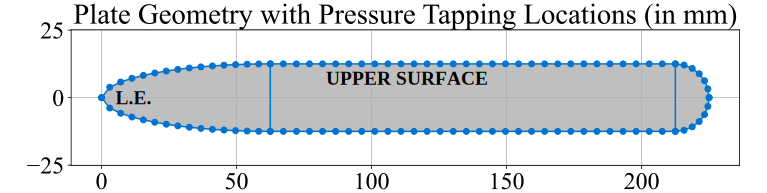
\includegraphics[width = \columnwidth]{exp_1_plate_geometry.png}
\caption{Plate geometry with pressure tapping locations (in mm).}
\label{exp_1_fig1}}
\end{figure}

Measurements were recorded digitally using a mixture of hardware and software. All time-averaged pressure data was captured by means of a 16-channel pneumatic pressure acquisition system, referred to as the DSA, which was controlled by a custom LabVIEW script. The DSA was set to record relative to $P_{atm}$ and, when required, could be connected to the necessary pressure tappings through polythene pipes and hypodermic tubing. A three-hole probe could be inserted into the wake traverse gear, which was also controlled by a LabVIEW script, in order to precisely capture pressure data downstream of the plate. Time-averaged temperature data was measured by means of a digital thermocouple which was connected to the computer via USB. A digital barometer was used to record the local atmospheric conditions.

The experimental procedure consisted of three activities: (1) surface pressure measurement, (2) probe calibration, and (3) wake traverse measurement. Each part of these activities is described in detail in the remainder of this section. 

\subsection{Activity 1}
The aim of the first activity was to use the low-speed wind tunnel to measure the surface pressure distribution around the flat plate. In order to achieve this, it was first necessary to determine the tunnel operating parameters and to configure the DSA. With the DSA connected to the reference pressure tappings and already gathering data, the wind tunnel was switched on and allowed to settle at its high-speed operating point. The data points collected by the DSA in the first 10 minutes, which were each the mean of 200 consecutive samples, were used to estimate a tunnel settling time for all future activities.

With the tunnel at its steady-state condition and the DSA still connected to reference tappings, with any spare channels connected to salient plate surface tappings, it was then necessary to determine the sample size over which the DSA should average. The DSA was set to capture 300 consecutive readings, each with a sample size of one, in order to gather enough data to plot standard deviation against sample size. An acceptable sample size was determined for future experiments as the minimum sample size that gives a low and relatively converged standard deviation.

The DSA was set to record at the new sample size thus making it possible to gather pressure data in an acceptable time frame without compromising accuracy. Pressure measurements were then recorded around the flat plate at all 104 tappings. It was necessary to dedicate two of the DSA channels to always measuring inlet stagnation and static pressures so as to have a consistent record of tunnel conditions; all remaining channels were used to gather data for tappings in parallel. Due to the abundance of tappings verus channels, these measurements were repeated for each tapping set until all tappings had been swept. The above procedure was then repeated at the low-speed operating condition having allowed the tunnel to re-settle in between measurements.

\subsection{Activity 2}
The aim of the second activity was to use the ‘Bingo Machine’ to generate yaw angle, stagnation pressure, and dynamic pressure relationships for the three-hole probe. In order to facilitate this, the probe had to be mounted on a rotary traverse gear with its head inserted directly in the middle of the main flow. The rotary traverse was controlled by means of a stepper motor, its driver, and a LabVIEW script. Only the probe-head and tunnel reference pressures were connected to the DSA. To achieve a high quality calibration, it was first necessary to determine the settling time of the system. This involved swinging the probe back and forth between relative incoming flow angles of -45 and +45\,$^\circ$, waiting a set period of time, then recording the pressures. Data points recorded at equal locations were compared for wait times of 0.1, 1.0 and 5.0 seconds. 

The DSA was set to record with an appropriate wait time and sample size, thus making it possible to gather pressure data in an acceptable time frame without compromising accuracy. The next step was to conduct both coarse and fine calibrations at the maximum wind tunnel flow speed of 45\,m/s. This involved traversing the probe from -45\,$^\circ$ to +45\,$^\circ$ (relative to the flow) and capturing pressure readings at each angular position. To obtain high fidelity measurements in the central region of interest, it was necessary to concentrate data points near 0 degrees yaw. The above calibration was simply repeated at the medium and low-speed operating conditions, with tunnel flow speeds of 27 and 12\,m/s respectively, in order to test for Reynold’s number effects. 

\subsection{Activity 3}
The aim of the third activity was to use the three-hole probe and wind tunnel traverse gear to perform a high resolution wake traverse at a distance of $C_x /3$ downstream of the flat plate trailing edge. In order to achieve this, both the probe and rotary traverse gear had to be mounted onto the main wind tunnel wake traverse gear; the rotary traverse was not removed from the probe so as to maintain any zero-offset error present in the calibration. The probe head was inserted at a distance of $s/2$ into the test section, i.e. at midspan of the plate, to minimise the impact of the endwall boundary layers. As before, the DSA was only connected to the reference tunnel inlet and probe-head pressures

With the traverse and probe setup complete, the wind tunnel was switched on and left to settle at its full-speed operating condition. The traverse gear then performed coarse and fine wake traverses, both controlled by means of a stepper motor and LabVIEW script, spanning roughly 3 plate thicknesses either side of the plate chord-line. Data points were concentrated (in the spanwise direction) downstream of the trailing edge in an attempt to more accurately resolve the shape and extent of the wake. The standard deviation test from the first activity was then repeated with the probe in the main flow, then in the wake,  to investigate the standard error of the probe. Lastly, the above procedure was simply  repeated at the low-speed operating condition, having allowed the tunnel to re-settle. 

\section{Results and Discussion}
\subsection{Surface Pressure Distribution}
A tunnel settling time of approximately 5 minutes was deemed appropriate based on pressure data captured in the first ten minutes of wind tunnel operation. It should be noted that the tunnel inlet temperature increases beyond this settling time, however, the absolute changes are small and thus the tradeoff between accuracy and time is favourable. 

Figure \ref{exp_1_fig2} plots standard deviation (std.devs) against sample size for the tunnel stagnation and static reference pressures, as well as for the flat plate leading and trailing edge pressures, measured at a chord-based Reynold’s number of $4.06\times 10^5$. Only data from these four channels is displayed due to the fact that the reference tappings remain connected for the entirety of the activity, and because the leading and trailing edges correspond to the minimum and maximum surface pressure std.devs respectively.

\begin{figure}[!ht]
{\centering
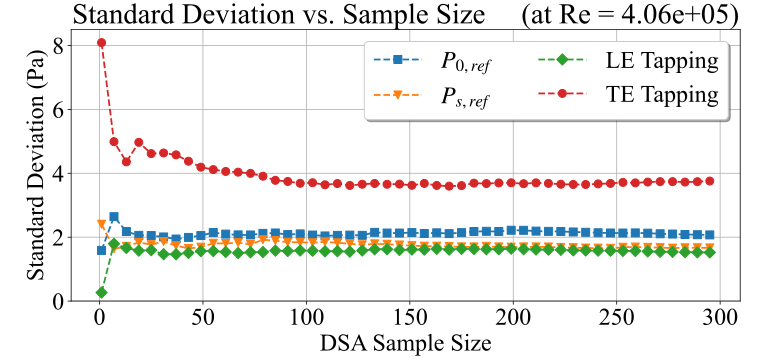
\includegraphics[width = \columnwidth]{exp_1_standard_deviation_pressure.png}
\caption{Standard deviation versus DSA sample size.}
\label{exp_1_fig2}}
\end{figure}

It is clear that for a DSA sample size of 200, the std.dev of each of the samples is converged with the error in the mean of each of the populations. In other words, an average pressure based on 200 consecutive samples is acceptable for all future activities. The std.dev in the reference pressures, each evaluated at a sample size of 200, were chosen to determine uncertainties involving reference pressure terms. The std.dev in the trailing edge pressure, also evaluated at a sample size of 200, was chosen as an upper bound for determining uncertainties involving any surface pressure terms. This combination guarantees that uncertainty intervals are fairly conservative. 

Figures <ref> and <ref> plot the surface static pressure coefficients against normalised axial chord position, for both the upper and lower surfaces of the flat plate, at chord-based Reynolds numbers of $1.82\times10^5$ and $4.03\times10^5$ respectively. Grey markers have been added to each plot to help identify the locations at which the plate’s geometry changes from elliptical to flat and circular. 95\% confidence bands have been derived and plotted for each dataset in order to present the overall uncertainty in $C_p$ due to bias and precision errors.  

\begin{figure}[!ht]
{\centering
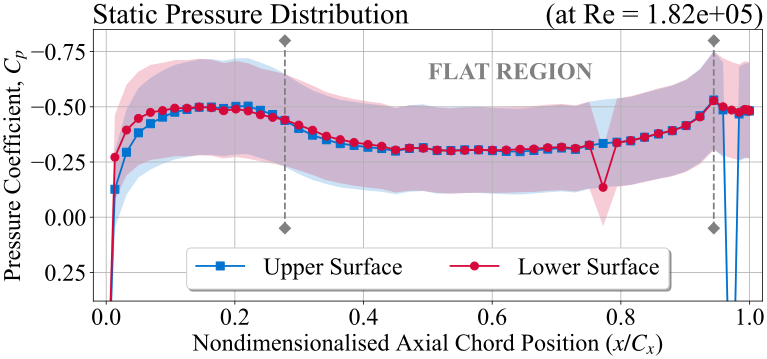
\includegraphics[width = \columnwidth]{exp_1_surface_pressure_dist_low_re.png}
\caption{$C_p$ distribution verus normalised axial chord at low-speed operation.}
\label{exp_1_fig3}}
\end{figure}

\begin{figure}[!ht]
{\centering
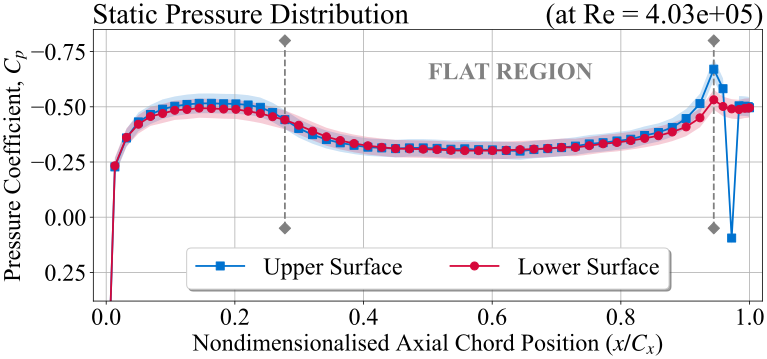
\includegraphics[width = \columnwidth]{exp_1_surface_pressure_dist_high_re.png}
\caption{$C_p$ distribution verus normalised axial chord at low-speed operation.}
\label{exp_1_fig4}}
\end{figure}

The first thing to note is that the upper and lower surface pressure distributions are practically identical in both figures. This shows that the average surface pressures acting on the skin of the plate are symmetric along the chord line and thus the aerofoil generates zero lift. It is important to remember that since these are time-averaged measurements, this does not imply in any way that the instantaneous pressure and velocities are symmetric. The second key finding is that the surface pressure distributions over the majority of the plate change very little with Reynolds number in the range tested; this simply implies that the experiment was not able to capture any Reynold’s number based effects on $C_p$. There are slight differences in $C_p$ between the upper and lower surfaces near the leading and trailing edges, but most of these lie within the accepted range of uncertainty. 

In terms of the shape of the distribution, the static pressure reduces along the elliptical section in a decreasing fashion. This is believed to be a result of boundary layer growth, a decreasing change in angularity of the pressure tappings, and an increase in blockage as the plate develops to its full thickness. The pressure then increases slightly and settles in the flat region; this implies that the boundary layer growth is slow and that the blockage does not increase considerably. The flow changes again in the circular section, perhaps due to a separation bubble, but it is unclear due to the lack of data points. The uncertainties in $C_p$ derived from measurements at the high-speed operating point are smaller than those derived for the low-speed operating point, simply due to the fact that the absolute gauge pressures are larger at higher speeds. 

\subsection{Three-Hole Probe Calibration}
There was no discernable difference in measurement when trying to determine the probe settling time. Although it was assumed that 0.1 seconds was sufficient, the DSA was set to wait for 1.0 second between successive measurements to be absolutely sure. Figures \ref{exp_2_fig1}, \ref{exp_2_fig2} and \ref{exp_2_fig3} show the calibration relationships obtained experimentally for yaw coefficient, stagnation pressure coefficient and dynamic pressure coefficient respectively, each for three Reynolds numbers. All of the curves are plotted with respect to relative oncoming flow angle (in degrees with clockwise defined as negative) since this was the primary dependent variable in the calibration activity. Once again, 95\% confidence bands have been derived and plotted for each Reynolds number for each dataset in order to present the overall uncertainty due to bias and precision errors. 

\begin{figure}[!ht]
{\centering
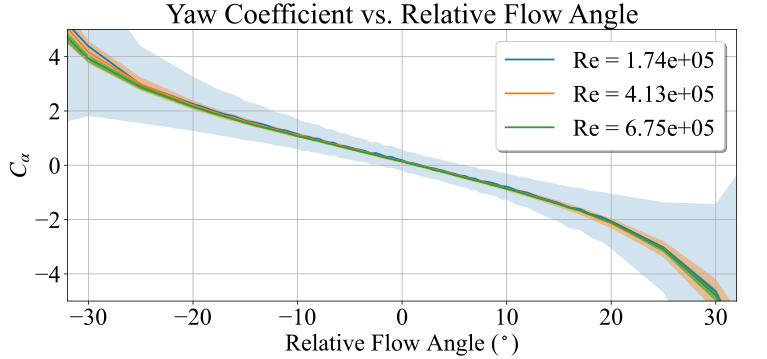
\includegraphics[width = \columnwidth]{exp_2_yaw_coefficient.png}
\caption{$C_\alpha$ obtained through calibration at high, medium and low Re.}
\label{exp_2_fig1}}
\end{figure}

\begin{figure}[!ht]
{\centering
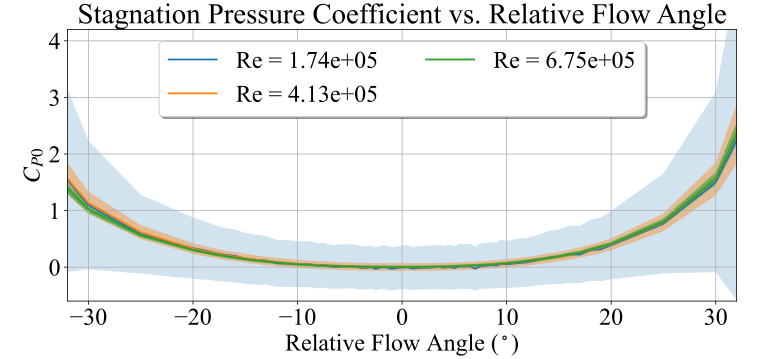
\includegraphics[width = \columnwidth]{exp_2_stg_coefficient.png}
\caption{$C_{P0}$ obtained through calibration at high, medium and low Re.}
\label{exp_2_fig2}}
\end{figure}

\begin{figure}[!ht]
{\centering
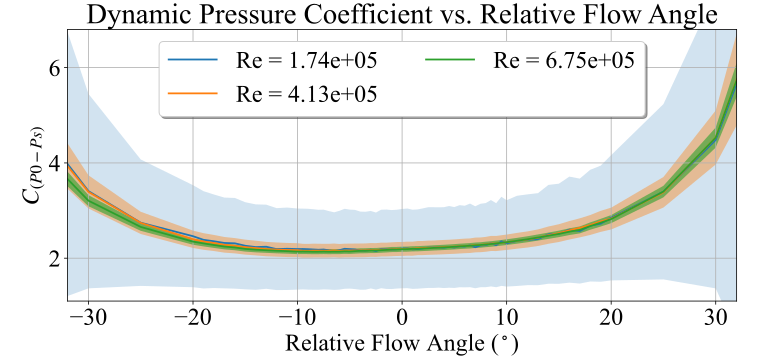
\includegraphics[width = \columnwidth]{exp_2_dyn_coefficient.png}
\caption{$C_{dyn}$ obtained through calibration at high, medium and low Re.}
\label{exp_2_fig3}}
\end{figure}

All three calibration relationships are as expected when compared to other low-speed three-hole probe calibrations discussed in the literature [cite]. In terms of shape, the yaw coefficient is clearly an odd one-to-one function of yaw angle in the range of Reynolds numbers tested. Generally speaking, this means that it can be relied on to produce the correct yaw angle when interpolating yaw coefficient in the wake traverse experiment. The other coefficients are clearly even many-to-one functions of yaw angle in the range of Reynolds numbers tested, however, this is not a problem since they are only used to interpolate based on the derived yaw angle itself. 

Perhaps the most significant observation is that, in each of the above three figures, the curves collapse on top of each other regardless of chord-based Reynolds number. This finding strongly implies that there are no Reynolds based effects in any of the calibrations in the range of the Reynolds numbers tested. Since the uncertainty is least in the high-Reynolds calibration curves, and since the range of testing includes both wind tunnel operating points, all three of these datasets are carried forward into wake traverse activity. In terms of gradients, in the linear region that exists between $\pm 20 ^\circ$ for yaw coefficient, the rate of change of $C_\alpha$ with respect to $\alpha$ is approximately -0.1. In the linear regions that exist between $\pm 10 ^\circ$ for the stagnation and dynamic pressure coefficients, the rate of change of $C_{P0}$ and $C_{P0 - Ps}$ are both very close to zero. 

\subsection{Wake Traverse}
The std.dev in the reference pressures, each evaluated at a sample size of 200, were chosen to determine uncertainties involving reference pressure terms. The std.dev in the probe-head pressure, also evaluated at a sample size of 200, were chosen for determining uncertainties involving any probe-head terms. This combination guarantees that uncertainty intervals are fairly accurate yet still conservative. Again, 95\% confidence bands have been derived and plotted for each dataset in order to present the overall uncertainty in due to bias and precision errors.

Figure \ref{exp_3_fig1} plots the wake traverse relative flow angle versus normalised traverse location for flow over a flat plate with chord-based Reynolds numbers of $1.75 \times 10^5$ and $3.88 \times 10^5$ respectively. Only the data points for the fine traverses are plotted. As before, 95\% confidence bands have been derived and plotted for each Reynolds number for each dataset in order to present the overall uncertainty due to bias and precision errors. The first thing to note is the rotational symmetry present in both curves; this implies that the average wake flow is symmetric about the chord-line of the plate. 

\begin{figure}[!ht]
{\centering
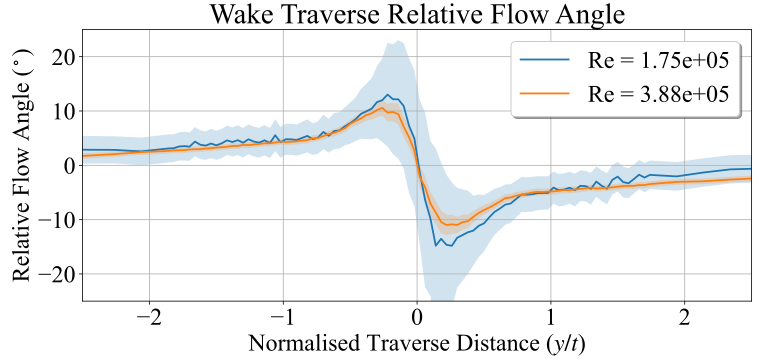
\includegraphics[width = \columnwidth]{exp_3_yaw_measurement.png}
\caption{Derived relative flow angle in the wake traverse.}
\label{exp_3_fig1}}
\end{figure}

It is clear that far from the trailing edge, the relative flow angles are small but non-zero: all relative flow angles are positive above the trailing edge whereas, below the trailing edge, all relative flow angles are negative. This either indicates that the flow everywhere is moving towards the chord-line or that there is an error in calibration. Unlike in the previous activities where there were no clear Reynolds based effects, it can now be seen that the peak turning angle is greater at the lower Reynolds number (12 vs. 10 $^\circ$). This makes sense relative to theory in that separation occurs more strongly behind circular trailing edges at higher Reynolds numbers. 

Figure \ref{exp_3_fig2} plots the wake traverse stagnation pressure loss coefficient versus normalised traverse location for flow over a flat plate with chord-based Reynolds numbers of $1.75 \times 10^5$ and $3.88 \times 10^5$ respectively. The data points at both wind tunnel operating conditions form highly symmetric bell-shaped distributions that span approximately 0.75 plate thicknesses either side of the chord-line. Clearly, based on the fact that both distributions have equal central-lobe widths, the extent of the wake is independent of Reynolds number in the range of Reynolds numbers tested. Although the peak values differ, most of the data points lie within the accepted range of uncertainty and thus it should be concluded that the intensity of entropy generation is independent of Reynolds number too. 

\begin{figure}[!ht]
{\centering
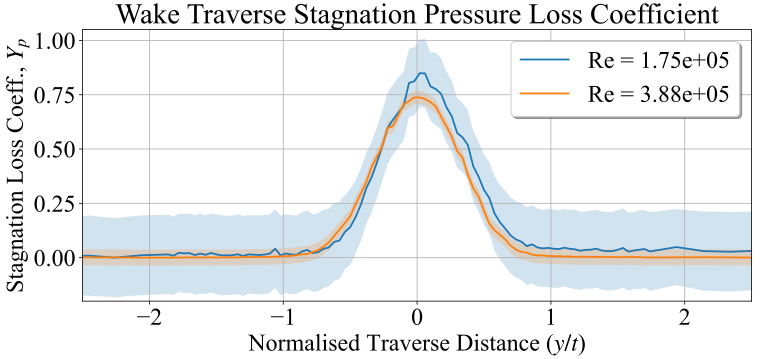
\includegraphics[width = \columnwidth]{exp_3_stag_loss_coefficient.png}
\caption{Derived stagnation pressure loss coefficient distribution.}
\label{exp_3_fig2}}
\end{figure}

The derived values of $Y_p$ for the outermost traverse locations, \textit{i.e.} the fringe regions surrounding the central wake, are essentially constant and fluctuate around zero. This implies that entropy creation rates in the main flow are negligible compared to the wake flow and that, in general, the core flow may be assumed isentropic. Contemporary cascade theory is aligned with this assessment as long as the blade aspect ratio does not significantly affect the assumption of two-dimensional potential flow. 

The mass averaged stagnation pressure loss coefficient is representative of the average losses generated by the flat plate aerofoil. Its value is defined as the mass weighted stagnation pressure loss flux, integrated over the wake traverse, divided by the local mass flux, also integrated over the wake traverse. Since it is impossible to capture data continuously, this quantity was evaluated by means of a second-order accurate trapezium rule integration scheme. Performing this calculation yields mass averaged stagnation pressure loss coefficients of 0.06959  and 0.05292 for the low-speed and high-speed tests respectively. This implies that the losses on the plate are higher at lower Reynold’s numbers. 

\section{Uncertainties}
In order to access the code used for plotting the figures and error bands shown in this report, as well as to access the data directly, please refer to this GibHub repository \href{https://github.com/RobertMichaelSales/FPP3-Interim-Report}{(Click Here!)}. The files within contain all uncertainty derivations in Python code form.

\section{Conclusions}
The aim of the experiment discussed in this report was to investigate the flow around a flat plate aerofoil using time-averaged data acquisition techniques. The experiment consisted of three activities: a surface pressure distribution measurement, a three-hole probe calibration, and a wake traverse experiment. Each of these activities required the use of steady pressure and temperature data acquisition hardware and software. Tests were conducted on the aerofoil at several Reynold’s numbers in order to determine any Reynolds number based effects. 

Results from the first activity show that the surface pressure distributions are symmetric about the chord-line of the aerofoil and that there are no discernable Reynolds effects. A flat plate aerofoil generates no lift by virtue of this symmetry. It was also shown that a DSA sample size of 200 was an acceptable compromise between experiment precision and experiment duration.

The calibration provided useful relationships between yaw coefficient, stagnation pressure coefficient and dynamic pressure coefficient versus relative flow angle; these were applied successfully to the measurement of the angularity and loss in the wake traverse. There were no Reynolds effects on the calibration relationships in the range tested. 

Finally, the wake traverse results show that the average wake flow is symmetrical about the chord-line, both in terms of entropy generation intensity and angularity. The extent of the wake was approximately 0.75 plate thicknesses either side of the chord-line for both Reynolds numbers tested. Again, this implies there are no Reynolds effects in the range tested. 



%\bibliographystyle{plain}
%\small
%\bibliography{CascadeExperiment.bib}
%============================================================================

\end{document}



%\title{Title}
%\author{Author}
%\maketitle

%\addcontentsline{toc}{section}{name}

%\begin{framed}
%\end{framed}

%\begin{table}[!ht]
%\begin{tabular}{l l l}
%\end{tabular}
%\end{table}

%\begin{table}[!ht]
%\begin{tabularx}{\textwidth}{l | X}
%\end{tabularx}
%\end{table}

%{\setlength{\extrarowheight}{1pt}
%}

%\multirow{rownumber}{*}{text} 
%\cline{2-5} --> A horizontal line for columns 2 to 5 for example

%\begin{equation} 
%\end{equation}

%\begin{itemize}
%\item Item
%\end{itemize}

%\begin{figure}[!ht]
%{\centering
%\includegraphics[height=]{}
%\caption{}
%\label{label_name}}					% ----> REFERENCE BY: \ref{name_of_reference}
%\end{figure}

%\begin{thebibliography}{99}
%\addcontentsline{toc}{section}{References}
%\bibitem{name_of_reference} 					 ----> CITE BY: \cite{name_of_citation}
%\end{thebibliography}